% !TeX program = lualatex
\documentclass[12pt,a4paper]{book}

% --- Grundpakete ---
\usepackage{fontspec}              % Unicode & Systemfonts (LuaLaTeX)
\usepackage[ngerman]{babel}        % Deutsche Sprache
\usepackage{amsmath,amssymb}       % Mathematische Symbole
\usepackage{graphicx}              % Bilder einfügen
\usepackage{listings}              % Quellcode-Umgebung
\usepackage{xcolor}                % Farben (statt 'color')
\usepackage{hyperref}              % klickbare Links
\usepackage{geometry}              % Seitenränder
\geometry{a4paper, margin=2.5cm}
\usepackage{float}                 % für [H]

\usepackage{tikz}
\usetikzlibrary{arrows.meta,calc,positioning}


\usepackage{titlesec}
\titleformat{\paragraph}[block]{\normalfont\normalsize\bfseries}{}{0pt}{}
\titlespacing*{\paragraph}{0pt}{1ex}{0.5ex}

% --- Schriften & Fallbacks (robust, mit IfFontExists) ---
% Hauptschrift: Noto Serif -> DejaVu Serif -> Latin Modern
\IfFontExistsTF{Noto Serif}{\setmainfont{Noto Serif}}{%
	\IfFontExistsTF{DejaVu Serif}{\setmainfont{DejaVu Serif}}{\setmainfont{Latin Modern Roman}}}

% Symbol-Fallback (z.B. U+25CC)
\IfFontExistsTF{Noto Sans Symbols 2}
{\newfontfamily\SymbolsFallback{Noto Sans Symbols 2}[Scale=MatchLowercase]}
{\newfontfamily\SymbolsFallback{DejaVu Sans}[Scale=MatchLowercase]}

% Arabisch
\IfFontExistsTF{Noto Naskh Arabic}
{\newfontfamily\arabicfont[Script=Arabic]{Noto Naskh Arabic}}
{\IfFontExistsTF{Amiri}{\newfontfamily\arabicfont[Script=Arabic]{Amiri}}{\newfontfamily\arabicfont[Script=Arabic]{Scheherazade}}}

% CJK (Chinesisch/Japanisch/Koreanisch) – wähle verfügbare Variante
\IfFontExistsTF{Noto Sans CJK SC}
{\newfontfamily\cjkfont{Noto Sans CJK SC}}
{\IfFontExistsTF{Noto Sans CJK JP}{\newfontfamily\cjkfont{Noto Sans CJK JP}}{\newfontfamily\cjkfont{DejaVu Sans}}}

% Emoji (farbig, falls vorhanden) -> sonst monochrom
\IfFontExistsTF{Noto Color Emoji}
{\newfontfamily\emojifont{Noto Color Emoji}[Renderer=Harfbuzz]}
{\IfFontExistsTF{Noto Emoji}{\newfontfamily\emojifont{Noto Emoji}}{\newfontfamily\emojifont{DejaVu Sans}}}

% Hilfsbefehle (z. B. dotted circle / kombinierender Akut)
\newcommand{\dottedcircle}{{\SymbolsFallback ◌}} % U+25CC
\newcommand{\combacute}{\char"0301}              % U+0301

% --- Listings-Einstellungen ---
\lstset{
	basicstyle=\ttfamily\small,
	keywordstyle=\color{blue}\bfseries,
	commentstyle=\color{gray},
	stringstyle=\color{red},
	numbers=left,
	numberstyle=\tiny,
	stepnumber=1,
	numbersep=5pt,
	frame=single,
	breaklines=true,
	captionpos=b
}

\begin{document}

\frontmatter
\title{Informatik-Skript für die E-Phase}
\author{[Jarek Mycan]}
\date{\today}
\maketitle

\tableofcontents

\mainmatter

\chapter{Einführung}
\section{Der Begriff Informatik}

Das Wort \textbf{Informatik} setzt sich aus zwei Teilen zusammen: \emph{Information} und \emph{Automatik}. 
Ursprünglich wurde der Begriff in den 1950er Jahren in Frankreich geprägt 
(\glqq informatique\grqq{}) und fand später auch im deutschsprachigen Raum Verbreitung. 
In anderen Sprachen wird der Bereich meist \glqq Computer Science\grqq{} genannt, 
was die technische Seite stärker betont. 

\subsection{Information}
Der erste Bestandteil, \emph{Information}, bezieht sich auf Daten, die eine Bedeutung tragen. 
Information ist also nicht einfach nur eine Ansammlung von Zeichen oder Zahlen, 
sondern sie entsteht erst durch die \emph{Interpretation} von Daten in einem bestimmten Kontext.  
Beispielsweise ist die Zahl \glqq 42\grqq{} zunächst nur ein einzelner Wert.
Wird sie jedoch im Zusammenhang mit einer Temperaturangabe, einem Alter oder einem Ergebnis verstanden, wird daraus eine Information.  
Die Informatik beschäftigt sich also damit, Informationen \emph{darzustellen}, 
\emph{zu speichern}, \emph{zu übertragen} und \emph{zu verarbeiten}.

\subsection{Automatik}
Der zweite Bestandteil, \emph{Matik} (von Automatik), bedeutet, dass diese Informationsverarbeitung 
durch Maschinen – insbesondere Computer – automatisiert geschieht.  
Ein zentrales Ziel der Informatik ist es, Verfahren zu entwickeln, die es ermöglichen, 
Informationen mithilfe von Computern effizient und zuverlässig zu verarbeiten. 
Dazu gehören das Erstellen von Programmen, das Entwerfen von Algorithmen 
sowie die Entwicklung von Systemen, die Informationen ohne manuelle Eingriffe verarbeiten können.

\section{Bedeutung der Informatik}
Die Informatik kann somit als \emph{Wissenschaft von der systematischen Verarbeitung von Informationen, insbesondere mit Hilfe von Computern}, verstanden werden. 
Sie ist nicht nur eine technische Disziplin, sondern verbindet Elemente aus 
Mathematik, Ingenieurwissenschaften, Logik und zunehmend auch Sozial- und Geisteswissenschaften. 
Heute prägt die Informatik nahezu alle Bereiche des täglichen Lebens: 
von Smartphones und dem Internet über moderne Autos bis hin zu Medizin, Wirtschaft und Wissenschaft.

\section{Was tun eigentlich Computer?}

Computer \emph{verarbeiten Daten}. Sie führen Berechnungen aus, speichern, übertragen und strukturieren Daten — aber sie „verstehen“ keine Bedeutung im menschlichen Sinn. Bedeutung (Information) entsteht erst beim Menschen (oder in einem Modell), wenn Daten in \emph{Kontext} gesetzt werden. Der Kernprozess ist daher zweistufig:

\begin{enumerate}
	\item \textbf{Repräsentation:} Aus \emph{Information} werden \emph{Daten}, indem wir festlegen, wie etwas als Zeichen/Zahlen (Bits) dargestellt wird.
	\item \textbf{Abstraktion:} Aus \emph{Daten} wird (wieder) \emph{Information}, indem wir Details weglassen, strukturieren und die Daten in einem Modell deuten.
\end{enumerate}

\subsection{Von Information zu Daten: Repräsentation}

\emph{Repräsentation} bedeutet: Wir legen eine \textbf{Abbildung} fest, die etwas Bedeutungsvolles (Information) in ein \textbf{Datenformat} überführt, das der Computer verarbeiten kann.
Formal kann man das als Funktion auffassen:
\[
\mathrm{rep}:\ \text{Information} \times \text{Kontext} \;\to\; \text{Daten (Bits)}.
\]


\subsection{Von Daten zu Information: Abstraktion}

\emph{Abstraktion} bedeutet: Wir \textbf{interpretieren} Daten in einem passenden Modell und \textbf{lassen Details weg}, die für die Fragestellung nicht nötig sind. So entsteht Bedeutung.
Formal:
\[
\mathrm{abs}:\ \text{Daten (Bits)} \times \text{Modell/Kontext} \;\to\; \text{Information}.
\]

\begin{figure}[H]
	\centering
	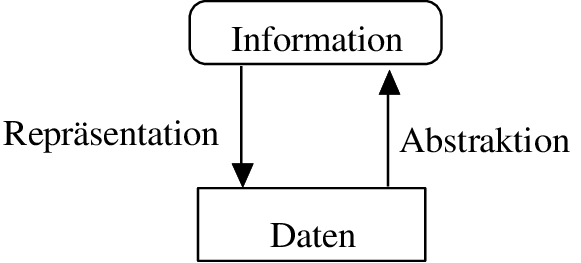
\includegraphics[width=0.55\textwidth]{info-daten.png}% ggf. Pfad anpassen
	\caption{Wechselspiel zwischen Repräsentation (Information → Daten) und Abstraktion (Daten → Information).}
	\label{fig:info-daten}
\end{figure}

\section{Bits und Bytes}

Ein \textbf{Bit} (binary digit) ist die kleinste Informationseinheit im Rechner: Es kann genau zwei Zustände annehmen, meist als \texttt{0} und \texttt{1} notiert. Physikalisch werden Bits z.\,B. durch zwei Spannungsniveaus, magnetische Ausrichtungen oder Lichtimpulse realisiert.

Einzelne Bits sind für die Verarbeitung jedoch zu fein. Deshalb werden Bits zu \textbf{Gruppen} zusammengefasst und \emph{gruppenweise} gelesen/geschrieben:

\begin{itemize}
	\item \textbf{Byte} = 8 Bit (heute die gebräuchlichste Grundeinheit; in den meisten Architekturen zugleich die \emph{kleinste adressierbare Einheit}).
	\item \textbf{Nibble} = 4 Bit (halbes Byte; nützlich z.\,B. bei Hexadezimaldarstellungen).
	\item \textbf{Wort (Word)} = \emph{architekturabhängige} Arbeitsbreite der CPU (typisch 16, 32 oder 64 Bit).
	\item \textbf{Doppelwort/Quadwort} = Vielfache der Wortbreite (z.\,B. 32/64/128 Bit).
\end{itemize}

\subsection{Wer bestimmt die Lesegruppen?}
\textbf{Hardware:} Die \emph{Register- und ALU-Breite} eines Prozessors legt fest, wie viele Bits er in einem Schritt besonders effizient verarbeiten kann (z.\,B. 32-Bit oder 64-Bit). Auch \emph{Datenbus} und \emph{Cache-Zeilengrößen} begünstigen das Holen/Speichern ganzer Bytes-, Wort- oder Mehrfach-Wort-Blöcke. Moderne CPUs können zusätzlich mit Vektor\-/SIMD-Einheiten noch größere Pakete (z.\,B. 128/256/512 Bit) auf einmal verarbeiten.

\textbf{Software/Betriebssystem:} Damit die Hardwarebreite genutzt werden kann, muss das \emph{Betriebssystem} die Architektur unterstützen (32-Bit- oder 64-Bit-Modus, Treiber, Systembibliotheken, ABI). Ein 64-Bit-Prozessor entfaltet seine Vorteile erst vollständig mit einem 64-Bit-Betriebssystem und passenden Programmen; andernfalls arbeitet er im 32-Bit-Kompatibilitätsmodus.

\paragraph{Beispiele.}
\begin{itemize}
	\item \textbf{32-Bit-System:} Die CPU arbeitet effizient mit 32-Bit-Wörtern (z.\,B. \texttt{int32}); Zeiger/Adressen sind 32 Bit breit. Daten werden häufig in 32-Bit-Schritten geladen/geschrieben, obwohl der Speicher byteweise adressiert wird.
	\item \textbf{64-Bit-System:} Register und Zeiger sind 64 Bit breit. Das System kann größere Zahlenbereiche adressieren und pro Schritt breitere Daten verarbeiten; trotzdem bleiben Bytes (8 Bit) die kleinste adressierbare Einheit.
\end{itemize}
\newpage
\section{Größe der Daten}

\begin{center}
	\begin{tabular}{r c l c l l}
		$1~\text{k}$ & = & $1024~\text{Bit}$ & = & $2^{10}$  & (k = Kilo)\\
		$1~\text{M}$ & = & $1024 \times 1024~\text{Bit}$ & = & $2^{20}$  & (M = Mega)\\
		$1~\text{G}$ & = & $1024 \times 1024 \times 1024~\text{Bit}$ & = & $2^{30}$  & (G = Giga)\\
		$1~\text{T}$ & = & $1024 \times 1024 \times 1024 \times 1024~\text{Bit}$ & = & $2^{40}$  & (T = Tera)\\
		$1~\text{P}$ & = & $1024 \times 1024 \times 1024 \times 1024 \times 1024~\text{Bit}$ & = & $2^{50}$  & (P = Peta)\\
		$1~\text{E}$ & = & $1024 \times 1024 \times 1024 \times 1024 \times 1024 \times 1024~\text{Bit}$ & = & $2^{60}$  & (E = Exa)\\
		$1~\text{Z}$ & = & $1024 \times 1024 \times 1024 \times 1024 \times 1024 \times 1024 \times 1024~\text{Bit}$ & = & $2^{70}$  & (Z = Zetta)\\
		$1~\text{Y}$ & = & $1024 \times 1024 \times 1024 \times 1024 \times 1024 \times 1024 \times 1024 \times 1024~\text{Bit}$ & = & $2^{80}$  & (Y = Yotta)\\
	\end{tabular}
\end{center}

\section{Textdarstellung}

\paragraph{Von ASCII zu Unicode — warum überhaupt?}
Frühe Computersysteme nutzten \textbf{ASCII} (American Standard Code for Information Interchange, 1960er Jahre). ASCII ist ein 7-Bit-Zeichensatz mit 128 Zeichen: lateinische Grundbuchstaben A–Z/a–z, Ziffern, Satzzeichen und Steuerzeichen (z.\,B. Zeilenumbruch). Für englischen Text genügte das, \emph{aber}:
Umlaute (ä, ö, ü), Akzente (é), das Euro-Zeichen (€), kyrillisch (Ж), griechisch (Ω), arabisch ({\arabicfont م}), asiatische Schriften ({\cjkfont 日}), Emojis ({\emojifont 😊}) \emph{fehlten}.
„é“ (NFC) vs. „e\combacute“ (NFD) bzw. „e + \dottedcircle\combacute“.
 \emph{fehlten}.


Als Übergang entstanden viele \textbf{„erweiterte ASCII“-Codepages} (8-Bit, 256 Zeichen), z.\,B. \texttt{ISO-8859-1}, \texttt{Windows-1252}, \texttt{KOI8-R}. Jede deckte \emph{einen} Sprachraum ab. Ergebnis: Inkompatibilitäten (sogenanntes \emph{Mojibake}), weil dieselben Bytewerte je nach Codepage andere Zeichen bedeuten.

\textbf{Unicode} (seit 1991) löst dieses Grundproblem: \emph{ein} weltweiter Zeichensatz für \emph{alle} Schriftsysteme, Symbole, technische Zeichen und Emojis. Ziel: \emph{„Jedem Zeichen ein eindeutiger Codepunkt“} — unabhängig von Sprache, Plattform oder Anwendung.

\paragraph{Begriffe sauber trennen}
\begin{itemize}
	\item \textbf{Codepunkt} (Unicode): eine Nummer in der Form \texttt{U+XXXX} (z.\,B. \texttt{U+00E4} = „ä“, \texttt{U+20AC} = „€“, \texttt{U+1F60A} = „😊“).
	\item \textbf{Kodierung} (Encoding): konkrete Regel, wie Codepunkte in \emph{Bytes} umgesetzt werden (z.\,B. UTF-8, UTF-16, UTF-32).
	\item \textbf{Graphem-Cluster}: was der Mensch als „ein Zeichen“ wahrnimmt (z.\,B. „e“ + kombinierender Akzent \texttt{U+0301} $\to$ „é“, oder Familien-Emoji aus mehreren Codepunkten).
\end{itemize}

\paragraph{Wichtige Unicode-Kodierungen}
\begin{itemize}
	\item \textbf{UTF-8} (variabel, 1–4 Byte pro Codepunkt): ASCII-Zeichen bleiben 1 Byte (abwärtskompatibel), alle anderen werden als 2–4 Byte kodiert. Heutzutage Standard im Web, in Dateien und Schnittstellen.
	\item \textbf{UTF-16} (variabel, 2 oder 4 Byte): Basis-Mehrsprachige Ebene (BMP) meist 2 Byte; Supplementärzeichen (z.\,B. viele Emojis) als Surrogatpaare (4 Byte). Achtung auf Byte-Reihenfolge (\emph{Endianness}) und optionales \emph{BOM}.
	\item \textbf{UTF-32} (fix 4 Byte): einfacher, aber speicherintensiv; praktisch v.\,a. intern in manchen Systemen.
\end{itemize}

\paragraph{Historische Entwicklung in Kürze}
\begin{description}
	\item[1963] ASCII (7-Bit) standardisiert Grundzeichen und Steuerzeichen.
	\item[1980er] Viele 8-Bit-Codepages (\texttt{ISO-8859-x}, \texttt{Windows-125x}) — regionale Lösungen, wenig kompatibel.
	\item[1991+] Unicode-Projekt: \emph{ein} universeller Zeichensatz; Trennung von \emph{Zeichen} (Codepunkte) und \emph{Kodierung} (UTFs).
	\item[2000er+] UTF-8 setzt sich global durch (Internet, Linux/Unix, moderne Apps und Protokolle).
\end{description}

\paragraph{Wie wird Unicode praktisch genutzt?}
\begin{itemize}
	\item \textbf{Dateien und Protokolle:} Textdateien, JSON, HTML, E-Mails, Datenbanken — fast überall ist UTF-8 üblich. Wichtig: \emph{Encoding angeben} (z.\,B. HTTP \texttt{Content-Type}, HTML \texttt{<meta charset="utf-8">}, DB-Kollation).
	\item \textbf{Betriebssysteme:} Dateinamen und Konsolen sind (je nach System) Unicode-fähig; moderne Terminals verstehen UTF-8.
	\item \textbf{Programmiersprachen:} Python, Java, JavaScript, C\# u.\,a. arbeiten intern mit Unicode-Zeichenketten; I/O nutzt meist UTF-8.
\end{itemize}

\chapter{Zahlensysteme}

\section{Was ist ein Zahlensystem?}
Ein \textbf{Zahlensystem} legt fest, wie Zahlen durch \emph{Ziffern} und deren \emph{Stellenwert} dargestellt werden.
In \emph{Stellenwertsystemen} (positionalen Systemen) hat jede Stelle einen Wert, der von der \emph{Basis} \(b\) abhängt:
\[
(d_k d_{k-1}\ldots d_1 d_0)_b
= d_k\cdot b^{k}+d_{k-1}\cdot b^{k-1}+\ldots + d_1\cdot b^1 + d_0\cdot b^0,
\]
wobei \(0 \le d_i < b\) gilt. Beispiele: Dezimal (\(b=10\)), Binär (\(b=2\)), Oktal (\(b=8\)), Hexadezimal (\(b=16\)).
Nicht-positionale Systeme (z.\,B. römische Zahlen) kennen keinen einheitlichen Stellenwert und sind für Rechenalgorithmen unpraktisch.

\section{Dezimalsystem (\(b=10\))}
Das \textbf{Dezimalsystem} nutzt die Ziffern \(0\)–\(9\).
Es ist heute \emph{weltweit das dominante System für den Alltag und das schulische Rechnen}.
Historisch hängt das vermutlich mit dem Zählen an zehn Fingern zusammen.
Beispiel:
\[
(5073)_{10} = 5\cdot 10^3 + 0\cdot 10^2 + 7\cdot 10^1 + 3\cdot 10^0.
\]

\section{Andere Zahlensysteme in der Welt}
\subsection*{Sexagesimalsystem (\(b=60\))}
Das \textbf{Babylonische Sexagesimalsystem} prägt uns bis heute: \emph{Zeitmessung} (60\,s \(=\) 1\,min, 60\,min \(=\) 1\,h) und \emph{Winkelmaße} (Grad–Bogenmaß mit Minuten und Sekunden). Rechnen erfolgt im Alltag dennoch meist dezimal; die Einteilung selbst ist aber sexagesimal.

\subsection*{Vigesimalsystem (\(b=20\))}
In Teilen der Welt gab und gibt es \textbf{Zwanzigersysteme} (Basis 20).
Sprachliche Spuren finden sich z.\,B. in Zahlwörtern einiger Sprachen (Restbestände wie „vier-mal-zwanzig“ für 80).
Auch hier wird formal in der Schule und in modernen Anwendungen überwiegend dezimal gerechnet.

\subsection*{Duodezimalsystem (\(b=12\))}
Das \textbf{Zwölfersystem} hat gute Teilbarkeit (2,3,4,6). Reste davon sieht man bei Dutzend/Groß, Uhren (12 Stunden), Maßeinheiten aus der Geschichte. Für maschinelles oder schulisches Rechnen dominiert aber 10.

\subsection*{Fazit zur Frage: „Rechnet man irgendwo ernsthaft nicht-dezimal?“}
\textbf{Menschen} rechnen heute fast überall \emph{dezimal}, mit kulturellen Resten anderer Basen in speziellen Domänen (Zeit, Winkel, Maße).  
\textbf{Maschinen} (Computer) \emph{rechnen binär}. Darauf basiert die Notwendigkeit weiterer Basen in der Informatik (Oktal/Hex als kompakte Binärdarstellung).

\section{Binär, Oktal, Hexadezimal – warum in der Informatik?}
\subsection*{Binärsystem (\(b=2\))}
Digitale Schaltungen kennen zwei stabile Zustände (z.\,B. „aus“/„ein“). Deshalb arbeitet Hardware \emph{binär}.
\[
(101010)_2 = 1\cdot 2^5 + 0\cdot 2^4 + 1\cdot 2^3 + 0\cdot 2^2 + 1\cdot 2^1 + 0\cdot 2^0 = 42.
\]

\subsection*{Oktalsystem (\(b=8\)) und Hexadezimalsystem (\(b=16\))}
Beide sind für Menschen \emph{kompakte Schreibweisen} von Binärzahlen:
\begin{itemize}
	\item 1 \textbf{Oktal-Ziffer} entspricht \textbf{3 Bit} (weil \(8=2^3\)).
	\item 1 \textbf{Hex-Ziffer} entspricht \textbf{4 Bit} (weil \(16=2^4\)).
\end{itemize}
Darum lassen sich Binärzahlen leicht gruppieren:
\[
\underbrace{1010}_{\text{A}}\,\underbrace{1010}_{\text{A}} = (\text{AA})_{16} = (10101010)_2.
\]
Hex ist heute Standard in Programmierung, Speicher-Dumps, Farbwerten (\#FF00AA), Adressen usw.
Oktal sieht man u.\,a. noch bei UNIX-Rechten (z.\,B. \(0755\)).

\section{Umrechnungen zwischen Basen}
\subsection*{Von Dezimal in eine Basis \(b\) (Divisionsrest-Methode)}
Beispiel: \(93_{10}\) nach Binär.
\[
\begin{array}{r|l}
	93:2 = 46 \text{ Rest }1\\
	46:2 = 23 \text{ Rest }0\\
	23:2 = 11 \text{ Rest }1\\
	11:2 = 5  \text{ Rest }1\\
	5:2  = 2  \text{ Rest }1\\
	2:2  = 1  \text{ Rest }0\\
	1:2  = 0  \text{ Rest }1
\end{array}
\Rightarrow\ (93)_{10} = (1011101)_2.
\]

\subsection*{Von Basis \(b\) nach Dezimal (Horner-Schema)}
Beispiel: \((2A)_{16}\) mit \(A=10\):
\[
(2A)_{16} = 2\cdot 16^1 + 10\cdot 16^0 = 32 + 10 = 42.
\]

\subsection*{Direkt zwischen Binär, Oktal, Hex}
Gruppieren in 3er- bzw. 4er-Blöcke (von rechts):
\[
(110\ 010\ 111)_2 = (627)_8,\qquad
(1010\ 1111)_2 = (\text{AF})_{16}.
\]

\section{Beispiele}
\begin{center}
	\begin{tabular}{r|c|c|c}
		\textbf{Dezimal} & \textbf{Binär} & \textbf{Oktal} & \textbf{Hex} \\
		\hline
		10 & \(1010\) & \(12\) & A \\
		26 & \(11010\) & \(32\) & 1A \\
		42 & \(101010\) & \(52\) & 2A \\
		64 & \(1000000\) & \(100\) & 40 \\
		100 & \(1100100\) & \(144\) & 64 \\
	\end{tabular}
\end{center}

\paragraph{Kleiner Blick über den Tellerrand.}
Auch andere Basen sind möglich und wurden erprobt (z.\,B. Ternär \(b=3\)).
Für die heutige Praxis gilt: Menschen bevorzugen \(b=10\), Computer arbeiten in \(b=2\); Oktal/Hex dienen als menschenfreundliche Brücke zur Binärwelt, Sexagesimal und Zwanziger-/Zwölfersysteme leben in speziellen Domänen weiter.

\section{Die Zweierkomplementdarstellung}

\subsection{Worum geht es?}
Computer speichern Zahlen als Bitmuster. Für \emph{positive} ganze Zahlen ist das einfach (normale Binärdarstellung). 
Aber wie speichern wir \emph{negative} Zahlen so, dass Addieren und Subtrahieren trotzdem mit der \emph{gleichen Hardware} funktionieren?
Die Antwort ist die \textbf{Zweierkomplementdarstellung}.

\subsection{Warum verwendet man das Zweierkomplement?}
\begin{itemize}
	\item \textbf{Ein Addierwerk für alles:} Dieselbe Schaltung addiert sowohl positive als auch negative Zahlen; Subtraktion wird als „Addiere das Zweierkomplement“ ausgeführt.
	\item \textbf{Eindeutige Null:} Es gibt nur \emph{eine} Null (anders als bei Vorzeichen-\&-Betrag oder Einerkomplement).
	\item \textbf{Einfache Regeln:} Vorzeichenverlängerung (Sign Extension) ist trivial: führende Einsen bei negativen Zahlen, Nullen bei positiven.
	\item \textbf{Sortier-/Vergleichsfreundlich:} Bei festem Wortbreite-Vergleich funktioniert das wie erwartet.
	\item \textbf{Mathematisch sauber:} Der Wertebereich ist genau \(-2^{n-1},\ldots,0,\ldots,2^{n-1}-1\) für \(n\)~Bit.
\end{itemize}

\subsection{So bildet man das Zweierkomplement (aus einer positiven Zahl \(x\))}
Für eine feste Wortbreite (z.\,B. 8~Bit):
\begin{enumerate}
	\item Schreibe \(x\) binär mit führenden Nullen.
	\item \textbf{Alle Bits invertieren} (0\,\(\leftrightarrow\)\,1).
	\item \textbf{+1 addieren.}
\end{enumerate}
Beispiel: \(-5\) als 8-Bit-Zahl. \\
\(+5 = \texttt{00000101}\ \Rightarrow\) invertiert \(\texttt{11111010}\ \Rightarrow\) \(+1\) \(\Rightarrow\) \(\boxed{\texttt{11111011}}\).

\subsection*{So liest man ein Zweierkomplement-Bitmuster}
\begin{itemize}
	\item \textbf{MSB (linkestes Bit) = 0} \(\Rightarrow\) positive Zahl: normal als Binärzahl lesen.
	\item \textbf{MSB = 1} \(\Rightarrow\) negative Zahl: wieder positiv machen durch \emph{invertieren + 1} und ein Minus davor.
\end{itemize}
Beispiel: \(\texttt{11101100}\) (8~Bit) \(\Rightarrow\) invertieren \(\texttt{00010011}\), \(+1\) \(\Rightarrow\) \(\texttt{00010100} = 20\) \(\Rightarrow\) Wert ist \(-20\).

\subsection*{Wertebereich}
Für \(n\)~Bit gilt:
\[
\boxed{\ -2^{n-1}\ \le\ \text{Wert}\ \le\ 2^{n-1}-1\ }\quad
\text{(z.\,B. 4~Bit: \(-8\) bis \(+7\)).}
\]
Auffällig: Es gibt \emph{kein} \(+2^{n-1}\) (bei 4~Bit also kein \(+8\)); das Muster \(\texttt{1000}\) steht für \(-8\).

\subsection*{Rechnen mit Zweierkomplement}
\paragraph{Addition/Subtraktion.}
\begin{itemize}
	\item Subtraktion \(a-b\) wird als \(a + (\text{Zweierkomplement von } b)\) gerechnet.
	\item \emph{Beispiel (4~Bit):} \(7 + (-3)\): \(\texttt{0111} + \texttt{1101} = \texttt{1 0100}\) \(\Rightarrow\) \(\texttt{0100} = 4\) (Übertrag links fällt weg).
\end{itemize}

\paragraph{Überlauf (Overflow) erkennen.}
\begin{itemize}
	\item \textbf{Regel:} Addiert man zwei \emph{positive} Zahlen und erhält eine \emph{negative}, oder zwei \emph{negative} und erhält eine \emph{positive}, dann ist Overflow aufgetreten.
	\item Alternativ technisch: Overflow, wenn \emph{Carry in} das Vorzeichenbit \(\neq\) \emph{Carry out} des Vorzeichenbits.
\end{itemize}

\paragraph{Vorzeichenverlängerung (Sign Extension).}
Erweitere eine Zweierkomplementzahl auf mehr Bit, indem du die \emph{linke führende Ziffer} wiederholst:
\begin{itemize}
	\item positiv: \(\texttt{0}\)en voran (z.\,B. \(\texttt{0010}\ \to\ \texttt{0000 0010}\))
	\item negativ: \(\texttt{1}\)en voran (z.\,B. \(\texttt{1110}\ \to\ \texttt{1111 1110}\))
\end{itemize}

\subsection*{Vergleich zu anderen Darstellungen}
\begin{description}
	\item[Vorzeichen \& Betrag:] Einfach zu verstehen (ein Bit fürs Vorzeichen), aber zwei Nullen (\(+0\) und \(-0\)) und Subtraktion ist umständlich.
	\item[Einerkomplement:] Auch zwei Nullen und kompliziertere Addition (End-Around-Carry).
	\item[Zweierkomplement:] \textbf{Standard in nahezu allen modernen CPUs} – schnell, eindeutig, hardwarefreundlich.
\end{description}

\subsection*{Beispiele (4-Bit)}
\begin{center}
	\begin{tabular}{c|r@{\qquad}c|r}
		\textbf{Bitmuster} & \textbf{Dezimal} & \textbf{Bitmuster} & \textbf{Dezimal} \\
		\hline
		\texttt{0111} & $+7$ & \texttt{1001} & $-7$ \\
		\texttt{0101} & $+5$ & \texttt{1011} & $-5$ \\
		\texttt{0000} & $0$  & \texttt{1111} & $-1$ \\
		\texttt{1000} & $-8$ & \texttt{1101} & $-3$ \\
	\end{tabular}
\end{center}


\subsection*{Abbildung}
\begin{figure}[H]
	\centering
	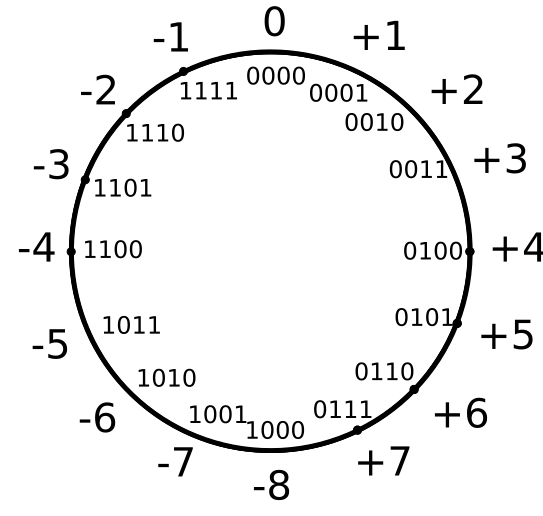
\includegraphics[width=.72\textwidth]{4Bit-2Komplement.png}
	\caption{4-Bit-Zweierkomplement: Zuordnung der Bitmuster zu Dezimalwerten und Bildung der negativen Werte (\(+1\) nach Bitinvertierung).}
	\label{fig:zweierkomplement-4bit}
\end{figure}

% Optional: kurze Übung (kannst du bei Bedarf aktivieren)
% \paragraph{Übung.}
% Wandle \(345_{10}\) in Binär, Oktal und Hex um.
% Prüfe: \(100_{10} = 84_{12}\) (Begründung).





\chapter{[Thema 1]}
\section{Grundlagen}
Hier beginnen wir mit deinem ersten Thema.

\chapter{[Thema 2]}
...

\backmatter
\chapter*{Anhang}
Quellen, Glossar, etc.

\end{document}

